\documentclass[11pt,letterpaper]{article}

% Publication-neutral, single-column research preprint.
% The original ICML manuscript remains in main.tex.
\usepackage[margin=1in]{geometry}
\usepackage[T1]{fontenc}
\usepackage{lmodern}
\usepackage{microtype}
\usepackage{graphicx}
\usepackage{booktabs}
\usepackage{array}
\usepackage{multirow}
\usepackage{xcolor}
\usepackage{amsmath,amssymb,amsfonts,amsthm,mathtools}
\usepackage{braket}
\usepackage{tikz}
\usetikzlibrary{positioning,arrows.meta,fit,shapes.geometric}

% Preserve the paper's existing \citep and \citet calls.
% plainnat prints author--year citations and an author--year bibliography.
\usepackage[authoryear,round]{natbib}
\usepackage[colorlinks=true,linkcolor=blue,citecolor=blue,urlcolor=blue]{hyperref}
\usepackage[capitalize,noabbrev]{cleveref}

\theoremstyle{plain}
\newtheorem{proposition}{Proposition}
\theoremstyle{remark}
\newtheorem{remark}{Remark}

% math_commands.tex — shared notation
\newcommand{\R}{\mathbb{R}}
\newcommand{\vz}{\mathbf{z}}
% readout support of qubit k at zero rotations, and the encoding angle
\newcommand{\Sk}{S_k}
\newcommand{\enc}[1]{a_{#1}}
% mean product order
\newcommand{\order}{\bar{s}}
% expectation value of Pauli-Z on qubit k
\newcommand{\ZZ}[1]{\langle Z_{#1}\rangle}
\newcommand{\pp}{\,pts}


\title{Products of Cosines: How the Entangling Layers of Quantum Classifier Heads\\
Shape the CNN Representations Trained Through Them}
% Set the public-facing author and affiliation before distribution.
\author{Alexander Greene}
\date{Research preprint \textemdash\ October 2026}

\begin{document}
\maketitle

\begin{abstract}
When a convolutional network is trained end to end through a variational quantum circuit
(VQC) classifier head, the head shapes the features the network learns. We measure this
effect with one common linear probe on the frozen 8-dimensional bottleneck of every trained
network. On CIFAR-10 with 4,000 training images, an 8-qubit VQC head with CNOT rings leaves
a bottleneck whose probe accuracy is 4.7 points below that of the same network trained with
a linear head (5 seeds, lower for every seed); removing the CNOT rings recovers 3.8 of those
points. An exact identity organizes the pattern: with every variational rotation at zero,
each readout is a product of cosines of the encoded inputs over a set fixed by the CNOT
layers. Across eleven circuit and classical heads, probe accuracy falls as the mean order of
these products rises, from 73.6 at order 1 to 69.8 at the default order 2.5 and 60.1 at
order 5.25. Classical heads trained on the same products, with no circuit, follow the same
trend, and a circuit that keeps its CNOTs but has product order 1 recovers 3.1 points.
Without CNOTs the head is exactly a classical per-coordinate sinusoidal model. Under a
revised protocol with longer training, validation-based selection and per-head
learning-rate tuning, the VQC's apparent advantage over a small MLP on MNIST shrinks from up
to 18 points to at most 3.3, and among linear, MLP and default VQC heads the linear head has
the highest mean test accuracy in all six settings.

\end{abstract}

\noindent\textbf{Keywords:} Quantum Machine Learning; Variational Quantum Circuits;
Representation Learning; Hybrid Models.

\section{Introduction}
\label{sec:intro}

A common near-term design for quantum image classification feeds a convolutional network
into a small variational quantum circuit (VQC) that acts as the classifier head
\citep{mari2020}, building on variational quantum classifiers
\citep{mitarai2018,havlicek2019,benedetti2019,cerezo2021}. When the network is trained jointly
\emph{through} the circuit, the head does more than classify: its gradients shape the
features the backbone learns. A comparison between a quantum head and a classical one
therefore compares two things at once, the heads and the representations they induce.
The question reaches beyond quantum machine learning: a head that distorts the features
trained through it is a known failure mode of fine-tuning \citep{kumar2022}, and here the
distortion turns out to track a structural quantity that can be computed before training.
Benchmarks of quantum classifiers typically score accuracy on fixed inputs
\citep[e.g.][]{fulton2026,slattery2022}; \citet{bowles2024} also replace the quantum layer of a trained
dressed hybrid network with a classical one and visualize how the learned layers transform
the data. Controls that isolate a circuit inside a hybrid model score predictive performance
\citep{kolle2024,elhag2026}. To our knowledge, none of these measures quantitatively what the quantum head
does to the representation trained through it, or which part of the circuit is
responsible.

We answer both questions for a CNN with an 8-dimensional bottleneck and an 8-qubit head
built from angle encoding $R_y(\pi\tanh z_j)$, four layers of trainable rotations each
followed by a ring of CNOTs, and a linear readout of $\ZZ{k}$. After joint training we
freeze each backbone and fit the same linear probe to its bottleneck, so that probe
accuracy compares the representations directly. The default VQC head lowers this probe
accuracy, and the size of the drop follows the circuit's CNOT structure. An exact identity
defines a structural descriptor whose order tracks this cost: when every trainable rotation
is zero, which is near where
training starts, each readout is
$\ZZ{k}=\prod_{j\in S_k}\cos(\pi\tanh z_j)$, a product of cosines over a set $S_k$ of
inputs fixed by the CNOT layers alone (\cref{fig:hero}a). The mean size of these sets, the
\emph{product order}, is 1 without CNOTs, 2.5 for the default circuit and 5.25 when a
single ring follows the last layer.

% Fig 1 (hero); panels (a, grids) and (b) from scripts/gen_fig1*.py, schematic drawn in fig1a_schematic.tex
\begin{figure*}[t]
  \centering
  % Fig 1a schematic: CNN -> bottleneck z -> 8-qubit VQC head -> linear readout, and the common
% linear probe on the frozen bottleneck. Requires tikz with positioning, arrows.meta, fit,
% shapes.geometric.
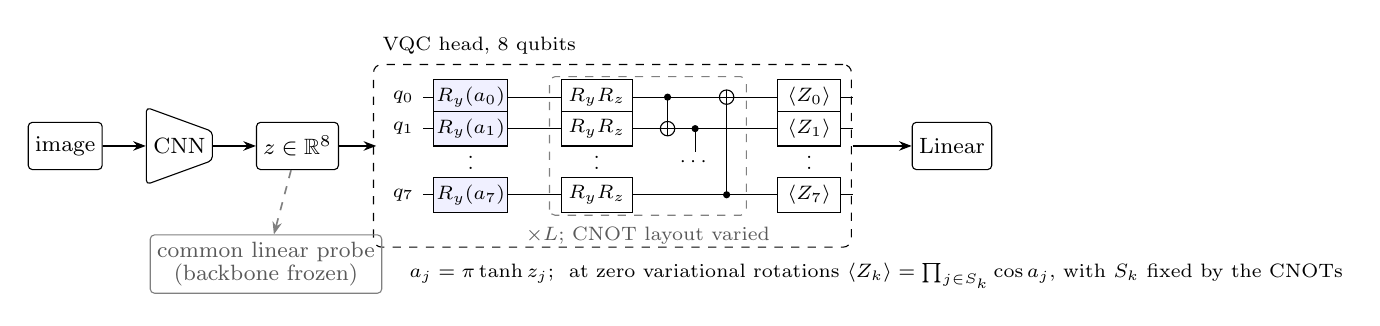
\begin{tikzpicture}[
    x=1cm, y=1cm, font=\footnotesize,
    box/.style={draw, rounded corners=1.5pt, minimum height=6mm, inner sep=2.5pt, align=center},
    gate/.style={draw, fill=white, minimum height=4.4mm, minimum width=9mm, inner sep=1pt, font=\scriptsize},
    arr/.style={-{Stealth[length=1.6mm]}, semithick},
  ]
  % classical front end
  \node[box] (img) at (0, 0) {image};
  \node[box, trapezium, trapezium angle=70, shape border rotate=270, minimum width=8mm] (cnn) at (1.45, 0) {CNN};
  \node[box] (z) at (2.95, 0) {$z\in\mathbb{R}^8$};
  \draw[arr] (img) -- (cnn);
  \draw[arr] (cnn) -- (z);
  \draw[arr] (z.east) -- (3.95, 0);

  % qubit wires q0, q1, ..., q7
  \foreach \y/\lab in {0.62/q_0, 0.22/q_1, -0.62/q_7} {
    \draw[thin] (4.55, \y) -- (10.0, \y);
    \node[font=\scriptsize, anchor=east] at (4.55, \y) {$\lab$};
  }
  \foreach \x in {5.15, 6.75, 9.45} \node[font=\scriptsize] at (\x, -0.18) {$\vdots$};

  % encoding R_y(a_j)
  \foreach \y/\j in {0.62/0, 0.22/1, -0.62/7}
    \node[gate, fill=blue!6] at (5.15, \y) {$R_y(a_{\j})$};

  % one variational layer: R_y R_z on every qubit, then a CNOT ring; repeated L times
  \foreach \y in {0.62, 0.22, -0.62}
    \node[gate] at (6.75, \y) {$R_y R_z$};
  \fill (7.65, 0.62) circle (1.3pt);                       % CNOT(0 -> 1)
  \draw (7.65, 0.62) -- (7.65, 0.22);
  \draw (7.65, 0.22) circle (2.6pt); \draw (7.65, 0.13) -- (7.65, 0.31);
  \fill (8.0, 0.22) circle (1.3pt);                        % CNOT(1 -> 2), down the ring
  \draw (8.0, 0.22) -- (8.0, -0.08);
  \node[font=\scriptsize] at (8.0, -0.2) {$\cdots$};
  \fill (8.4, -0.62) circle (1.3pt);                       % CNOT(7 -> 0) closes the ring
  \draw (8.4, -0.62) -- (8.4, 0.62);
  \draw (8.4, 0.62) circle (2.6pt); \draw (8.4, 0.53) -- (8.4, 0.71);
  \draw[dashed, rounded corners=2pt, gray] (6.15, -0.88) rectangle (8.65, 0.88);
  \node[font=\scriptsize, gray!70!black, anchor=north] at (7.4, -0.9) {$\times L$; CNOT layout varied};

  % measurement
  \foreach \y/\k in {0.62/0, 0.22/1, -0.62/7}
    \node[gate, minimum width=8mm] at (9.45, \y) {$\langle Z_{\k}\rangle$};

  % head frame and readout
  \node[draw, dashed, rounded corners=3pt, fit={(3.95, 1.0) (9.95, -1.25)}, inner sep=1pt,
        label={[font=\scriptsize, anchor=south west]north west:VQC head, 8 qubits}] (head) {};
  \node[box, anchor=west] (lin) at (10.75, 0) {Linear};
  \draw[arr] (10.0, 0) -- (lin.west);

  % zero-rotation identity
  \node[font=\scriptsize, anchor=west] at (4.25, -1.65)
    {$a_j=\pi\tanh z_j$;\ \ at zero variational rotations
     $\langle Z_k\rangle=\prod_{j\in S_k}\cos a_j$, with $S_k$ fixed by the CNOTs};

  % common linear probe on the frozen bottleneck
  \node[box, draw=gray, text=gray!70!black] (probe) at (2.55, -1.5) {common linear probe\\[-1pt](backbone frozen)};
  \draw[arr, dashed, gray] (z) -- (probe);
\end{tikzpicture}
\\[3mm]
  \begin{minipage}[c]{0.36\textwidth}
    \centering
    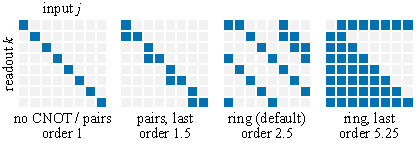
\includegraphics[width=\linewidth]{figures/fig1a_supports.pdf}\\[1mm]
    {\small (a)}
  \end{minipage}\hfill
  \begin{minipage}[c]{0.60\textwidth}
    \centering
    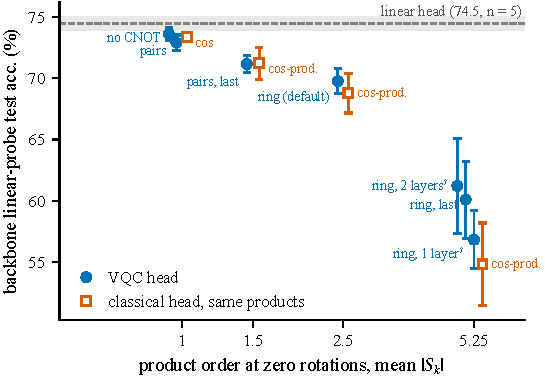
\includegraphics[width=\linewidth]{figures/fig1b_probe_vs_order.pdf}\\
    {\small (b)}
  \end{minipage}
  \caption{\textbf{(a)} A CNN feeds an 8-dimensional bottleneck $z$ into an 8-qubit VQC head
  (default: four $R_yR_z$ layers, each followed by a CNOT ring $(q, q{+}1 \bmod 8)$; variants
  place CNOTs after the last layer only (``last''), use $L\in\{1,2\}$ layers, or replace the ring
  by disjoint pairs $(0,1),(2,3),(4,5),(6,7)$). With every variational rotation at zero, each
  readout is exactly $\langle Z_k\rangle=\prod_{j\in S_k}\cos(\pi\tanh z_j)$; the grids mark
  $j\in S_k$ in blue (rows: readouts $k$, columns: inputs $j$). Pairs after every layer cancel
  at zero rotations, so their supports equal the no-CNOT ones. Product order is
  $\frac18\sum_k|S_k|$. The backbone is evaluated by one common linear probe on the frozen
  bottleneck. \textbf{(b)} CIFAR-10 with 4,000 training images: probe test accuracy against
  product order (log axis) for VQC heads (filled) and classical heads trained end to end on the
  zero-rotation products of a circuit (open; at order 5.25 these are the supports of ``ring,
  last'' and ``ring, 1 layer''; ``ring, 2 layers'' has different supports of the same mean
  order). Mean $\pm$ SD over 5 seeds ($\dagger$: 3); head learning rate selected on mean
  validation accuracy over seeds 0--2, seeds 3--4 run at that choice. Dashed line and band:
  linear head. Points at one order are offset horizontally. The plot shows an association;
  order co-varies with support overlap. Open diamonds: six CNOT layouts outside the ring family (5 seeds, \cref{app:family}),
  whose probe accuracy was predicted before training from the dotted fit over the ring-family (seeds 0--2)
  VQC circuits (linear in order, hence curved on the log axis); brickwork lies 5 points above its prediction. Open triangles: a CZ ring (entangling, order 1) and the CNOT-free circuit read out with $Z_kZ_{k+1}$ or $Z_kZ_{k+1}Z_{k+2}$ (orders 2 and 3), pre-registered, 5 seeds (\cref{tab:generality}).}
  \label{fig:hero}
\end{figure*}


Our contributions are:
\begin{enumerate}
  \item \textbf{A tuning audit} (\cref{sec:tuning}). Under a revised protocol (longer
        training, validation-based selection, each head's learning rate tuned), the VQC's
        apparent advantage over a near-parameter-matched MLP on MNIST shrinks from up to 18
        points to a largest observed mean of 3.3. On CIFAR-10 the VQC still trails the MLP by 3.1--9.2 points,
        and among the linear, MLP and default VQC heads the linear head has the highest mean
        test accuracy in all six dataset--size settings.
  \item \textbf{A representation cost tied to the CNOT layers} (\cref{sec:gap,sec:ring}). On
        CIFAR-10 with 4,000 training images the default VQC head lowers bottleneck probe
        accuracy by $4.7\pm0.9$ points relative to a linear head (5 seeds), and a two-layer
        MLP probe finds the same gap, so the loss is not just one of linear readability. Removing the CNOT
        rings recovers $3.8\pm1.2$ points. On a pretrained ResNet-18 the default head costs
        6--8 points at 1,000 to 10,000 images at an approximately matched number of updates (22.3 at 1,000
        with a fixed 30 epochs); the ring-free head stays within 1.4 points of linear
        (\cref{sec:pretrained}). Five controls leave a substantial gap
        (\cref{sec:controls}).
  \item \textbf{A structural account} (\cref{sec:order,sec:sinusoid}). Probe accuracy falls
        with product order across eleven heads (\cref{fig:hero}b). Classical heads trained
        on a circuit's zero-rotation products, with no circuit, follow the same trend; on the
        small CNN the default circuit's products match the VQC ($-1.0\pm2.2$), and on the
        pretrained backbone they reproduce the ordering.
        The ordering replicates on MNIST and on six new layouts (Spearman $-0.89$, two rank reversals), under predictions logged
        before but committed after those runs (\cref{app:repro}), and under committed predictions with a second encoding ($-0.94$) and at 12 qubits. A circuit that keeps its CNOTs
        but has product order 1 recovers $3.1\pm1.2$ points over the default. Entangling gates alone do not set the size of the cost here: a CZ ring, which entangles at order 1, probes 0.4 points below the ring-free head, and two- and three-body readouts of a circuit with no entangling gate land about 0.1 points from the order trend (\cref{tab:generality}).
        Without entangling gates and with single-qubit readouts the head is exactly a classical per-coordinate sinusoidal model, and
        classical heads of that form come within 0.3--0.9 probe points of it.
  \item \textbf{A mechanism} (\cref{sec:saturation}). We prove that, for independent inputs, a high-order product readout that keeps its magnitude must push its inputs out of the graded middle of the encoding (a signal budget),
        and find that the CNNs' bottlenecks saturate early and stay saturated at high order. A
        pre-registered intervention that leaves the forward pass unchanged but lets saturated
        coordinates escape recovers 6.8 of the 13.5 last-ring points; the order cost that remains, and an unbounded encoding that keeps two thirds of the slope, are consistent with the budget.
\end{enumerate}


\section{Related Work}
\label{sec:related}

\paragraph{Benchmarking quantum classifiers and the role of entanglement.}
Large benchmarks find that simple classical models generally match or beat variational
quantum classifiers, and that removing entanglement often does not hurt
\citep{bowles2024}; quantum fidelity kernels show a similar lack of advantage on classical
data \citep{slattery2022}. Closest to our setting, \citet{fulton2026} show that classical
$\mathrm{SU}(2)$ models match or exceed shallow VQCs on vision benchmarks and that ring
entanglement can degrade accuracy on fixed features. Recent hybrid-network studies reach
related conclusions under more careful matching of width and budget
\citep{freinberger2026,innan2026,park2026}. Other work trains hybrid models end to end and
studies the learned representation: \citet{kashif2026} analyze expressibility and
trainability under joint training, and quantum self-supervised learning evaluates frozen
hybrid encoders with linear probes \citep{jaderberg2021,edwards2026}. We probe the
supervised bottleneck \emph{before} the circuit, the representation the circuit's
gradients shape, and relate its accuracy to a quantity, product order, read off the CNOT
pattern.

\paragraph{Isolating the circuit inside hybrid models.}
A growing line of work asks what the quantum part of a hybrid model contributes.
\citet{kolle2024} separate classical and quantum contributions in hybrid architectures,
building on sequential training that first fits a classical surrogate and then swaps in the
circuit \citep{altmann2023}. \citet{elhag2026} delete, freeze or corrupt the circuit in
quantum message passing and compare it with exact classical surrogates under the same
$\pi\tanh$-style angle encoding. Data-encoding choices in hybrid convolutional models have
also been compared directly \citep{monnet2024}. These controls score predictive accuracy. We
add a representation-level measurement, a common probe on the jointly trained bottleneck,
and controls that change one structural property of the circuit at a time.

\paragraph{Fourier structure, classical surrogates and head-induced feature distortion.}
Angle-encoded circuits compute truncated Fourier series of their inputs
\citep{schuld2021,perez2020}, which classical models can represent and emulate
\citep{schreiber2023}; sinusoidal features also appear in classical networks as periodic
activations and Fourier feature maps \citep{sitzmann2020,tancik2020}. Our zero-rotation
identity is an elementary instance of this structure, used as an explanatory variable: it
shows which products the CNOT layers create, and their order tracks a measured cost. In classical deep learning, \citet{kumar2022} show that the
head used during fine-tuning distorts pretrained features, and linear probes are a standard
tool for reading what an intermediate layer encodes \citep{alain2017}. We apply the probe
to the quantum-head setting, where the head is a fixed-form circuit rather than a learned
classical layer.

\paragraph{Position of this work.}
That entanglement often does not help, and that trigonometric surrogates can stand in for
simple circuits, are known. What is new here is (i) a measurement of the bottleneck a
quantum classifier head induces under supervised joint training, with a probe shared across
quantum and classical heads, and (ii) a
structural variable, the order of the zero-rotation cosine products, that orders the
representation cost across circuit and classical heads and survives an intervention that
keeps entanglement while lowering order.

\section{Setup}
\label{sec:setup}

\paragraph{Model.}
A CNN backbone maps an image to a bottleneck $\vz\in\R^8$ (MNIST: three convolutional
blocks, about 94K parameters; CIFAR-10: four blocks, about 0.96M). Each head is trained
jointly with its own copy of the backbone. The \emph{linear} head is a single dense layer
(90 parameters); \emph{MLP-8} has one hidden layer of width 8 with ReLU (162). The default
\emph{VQC} head encodes $\enc{j}=\pi\tanh z_j$ by $R_y(\enc{j})$ on qubit $j$, applies $L=4$
layers of trainable $R_y R_z$ rotations on every qubit, each followed by a ring of CNOTs
$(q,q{+}1 \bmod 8)$ applied in order $q=0,\dots,7$, measures $\ZZ{k}$ on every qubit, and
maps the eight expectations to ten logits with a linear layer (154 stored parameters, 146
of which can affect the output). Rotations are initialized in $\mathcal{U}(-0.1,0.1)$. We
simulate the circuit exactly with a batched PyTorch statevector simulator that matches
PennyLane \citep{bergholm2018} to $10^{-6}$ in outputs and input gradients and $10^{-5}$ in
rotation gradients (our test suite). Circuit variants change CNOT placement or rotation
depth: \emph{no CNOT}; a ring after the \emph{last} layer only; $L\in\{1,2\}$
layers; and disjoint \emph{pairs} $(0,1),(2,3),(4,5),(6,7)$ after every layer or after the
last layer only.

\paragraph{Protocol.}
Training subsets are class-stratified samples of 250, 500 or 1,000 MNIST images and 1,000,
2,000 or 4,000 CIFAR-10 images; a disjoint stratified 2,000-image validation set selects
the checkpoint epoch. Every run uses AdamW (weight decay $10^{-4}$), a cosine schedule,
batch size 32 and gradient clipping, for 50 epochs on MNIST and 80 on CIFAR-10 with
standard augmentation. The backbone learning rate is half the head learning rate. For each
dataset, size and head we select the head learning rate with the best mean validation
accuracy over seeds 0--2 from a grid of half-decade steps, and report test accuracy once.
Headline CIFAR-10/4,000 cells add seeds 3 and 4 at that selected rate. Heads in a cell share
seeds, hence training subsets and validation splits, so we report paired differences
(mean $\pm$ SD over seeds, in percentage points). Every table states its number of seeds.

\paragraph{Common linear probe.}
To compare representations, we freeze each selected run's backbone, extract $\vz$ on clean
images, and fit a fresh linear layer $\R^8\to\R^{10}$ (AdamW, cosine schedule, probe
learning rate and epoch selected on validation). Because the probe is the same for every
backbone, differences in its test accuracy compare the bottlenecks that different heads
induced in joint training. We call this \emph{probe accuracy}.

\paragraph{Zero-rotation identity.}
With every trainable rotation set to zero, the variational block reduces to its CNOTs. The
encoded state is a product state with $\langle Z_j\rangle=\cos\enc{j}$, and conjugating by
$\mathrm{CNOT}(c,t)$ maps $Z_t\mapsto Z_cZ_t$ and leaves $Z_c$ unchanged. Propagating $Z_k$
back through the gates in reverse order, and cancelling repeated factors with $Z^2=I$, gives
a Pauli-$Z$ string on a set $\Sk$ of qubits:
\begin{equation}
  \ZZ{k}\big|_{\theta=0}=\prod_{j\in\Sk}\cos(\pi\tanh z_j),
  \qquad
  \order=\tfrac{1}{8}\textstyle\sum_{k}|\Sk| .
  \label{eq:identity}
\end{equation}
We call $\order$ the \emph{product order}. It is 1 without CNOTs, 2.5 for the default
circuit, 5.25 for a ring after the last layer or a single-layer circuit, 1.5 for pairs after
the last layer, and 1 for pairs after every layer: the pair layer $P$ satisfies $P^2=I$, so its four
copies cancel at zero rotations, while interleaved nonzero rotations generally prevent the
cancellation (\cref{fig:hero}a; \cref{app:identity} lists the supports). Without
CNOTs the identity extends to all rotation angles: each qubit evolves alone, so
\begin{equation}
  \ZZ{j}=\alpha_j\cos\enc{j}+\beta_j\sin\enc{j},
  \label{eq:ringfree}
\end{equation}
with $\alpha_j,\beta_j$ set by qubit $j$'s trained rotations. With its readout layer, the
ring-free head is thus a classical per-coordinate sinusoidal model (we checked the formula
against the simulator to $10^{-7}$). To test whether the products themselves carry the effect, we train classical
heads on them with no circuit: \emph{cos} uses $\cos\enc{j}$ (order 1), \emph{cos+sin} adds
$\sin\enc{j}$, and \emph{cos-prod.} uses the products of \cref{eq:identity} for a given
circuit's supports, each followed by a linear layer and tuned like every other head.

\section{Tuning Changes Head Comparisons, but a Linear Head Stays Ahead}
\label{sec:tuning}

\begin{table}[t]
\centering
\caption{Test accuracy (\%) of three heads on the same CNN, each with its head learning rate
selected by mean validation accuracy over the tested grid (backbone lr is coupled at $0.5\times$
the head lr); mean $\pm$ SD over 3 seeds; bold: highest mean in the row. MLP-8: one hidden
layer of width 8; VQC: the default 8-qubit, 4-layer ring circuit. Differences are in
percentage points, paired over seeds (same training subset and split). The last column
repeats VQC $-$ MLP-8 with both heads at one shared head lr ($10^{-3}$). The linear head's
selected lr lies at the top of its grid in five rows, so its lead may be understated.}
\label{tab:matched}
\small
\setlength{\tabcolsep}{4pt}
\begin{tabular}{llcccccc}
\toprule
& & \multicolumn{3}{c}{Selected lr} & \multicolumn{2}{c}{VQC $-$ (selected lr)} & VQC $-$ MLP-8 \\
\cmidrule(lr){3-5}\cmidrule(lr){6-7}\cmidrule(lr){8-8}
Data & $N_\mathrm{train}$ & Linear & MLP-8 & VQC & Linear & MLP-8 & (lr $10^{-3}$) \\
\midrule
\multirow{3}{*}{MNIST} & 250 & $\mathbf{90.3 \pm 1.9}$ & $78.7 \pm 6.5$ & $76.6 \pm 5.3$ & $-13.7 \pm 5.9$ & $-2.1 \pm 9.7$ & $+10.8 \pm 13.9$ \\
 & 500 & $\mathbf{94.3 \pm 0.2}$ & $86.7 \pm 3.0$ & $90.0 \pm 0.6$ & $-4.3 \pm 0.5$ & $+3.3 \pm 2.6$ & $+6.1 \pm 11.6$ \\
 & 1000 & $\mathbf{96.4 \pm 0.5}$ & $93.9 \pm 0.8$ & $94.6 \pm 0.4$ & $-1.7 \pm 0.9$ & $+0.8 \pm 1.0$ & $-0.5 \pm 3.8$ \\
\midrule
\multirow{3}{*}{CIFAR-10} & 1000 & $\mathbf{59.0 \pm 0.9}$ & $52.3 \pm 1.8$ & $43.1 \pm 3.8$ & $-15.8 \pm 3.8$ & $-9.2 \pm 4.5$ & $-13.6 \pm 1.8$ \\
 & 2000 & $\mathbf{67.6 \pm 0.7}$ & $62.0 \pm 1.0$ & $53.1 \pm 0.9$ & $-14.5 \pm 1.3$ & $-8.9 \pm 1.7$ & $-13.5 \pm 2.0$ \\
 & 4000 & $\mathbf{74.6 \pm 0.5}$ & $70.8 \pm 0.5$ & $67.7 \pm 1.1$ & $-7.0 \pm 1.2$ & $-3.1 \pm 0.9$ & $-10.1 \pm 1.6$ \\
\bottomrule
\end{tabular}
\end{table}


Before turning to representations, we check how much a head comparison depends on the training
recipe. With one shared recipe (head learning rate $10^{-3}$, 25 MNIST epochs; \cref{app:sweep}), the
VQC beat MLP-8 on MNIST by up to 18 points and lost to it on CIFAR-10 by 8--14. Under the protocol of
\cref{sec:setup}, these differences change in size and sign (\cref{tab:matched}): on MNIST, VQC
$-$ MLP-8 becomes $-2.1\pm9.7$, $+3.3\pm2.6$ and $+0.8\pm1.0$ at 250, 500 and 1,000 images, partly
through the protocol itself and partly through per-head tuning (last column); on CIFAR-10 the deficit
shrinks to 3.1--9.2 points. A linear head has the highest mean in all six settings and beats the VQC
for every seed. Every selected rate is interior to its grid.

This audit fixes the comparisons used in the rest of the paper: every head is evaluated at
its own validated learning rate. It also leaves a question. At 4,000 CIFAR-10 images the
VQC trails the linear head by $7.0\pm1.2$ test points (5 seeds: $6.7\pm1.0$). Part of that
gap could come from the VQC as a readout and part from the backbone it trains; a common probe
measures the gap that remains under one readout.

\section{What the VQC Head Does to the Backbone}
\label{sec:backbone}

\subsection{The default VQC head lowers bottleneck probe accuracy}
\label{sec:gap}

On CIFAR-10 with 4,000 images, the common probe reaches $69.8\pm1.0$ on backbones trained
with the default VQC head and $74.5\pm0.5$ on backbones trained with a linear head, a paired
difference of $-4.7\pm0.9$ points that is negative for all five seeds. The probe reads the
VQC-trained bottleneck better than the VQC head itself does ($67.8\pm1.3$ test): replacing
the VQC head by the probe raises accuracy by about 2.0 points, and a 4.7-point gap remains
between the two backbones under the common probe. The gap is larger with less data (CIFAR-10:
$-11.2\pm4.0$ and $-11.1\pm1.5$ at 1,000 and 2,000 images) and smaller on MNIST ($-7.9\pm4.2$,
$-2.2\pm0.8$ and $-1.0\pm0.5$ at 250, 500 and 1,000; 3 seeds each). A narrow classical head
lowers probe accuracy as well: MLP-8 backbones probe $3.6\pm0.6$ points below linear-head
backbones on CIFAR-10/4,000, $1.0\pm0.9$ above the VQC. The rest of this section shows that
the VQC's share of the gap depends on its CNOT structure, which no classical head has.

\subsection{Removing the CNOT rings recovers most of the gap}
\label{sec:ring}

Deleting every CNOT and keeping the rest of the head unchanged raises probe accuracy to
$73.6\pm0.5$ and test accuracy to $73.1\pm0.5$ (5 seeds). Against the default VQC this is
$+3.8\pm1.2$ probe and $+5.2\pm1.4$ test points, positive for every seed, and the ring-free
head now probes $2.8\pm0.6$ points above MLP-8. It leaves $0.8\pm0.5$ probe and $1.4\pm0.5$
test points to the linear head. MNIST shows the same direction: ring removal gains
$2.8\pm0.4$ and $1.4\pm0.4$ probe points at 500 and 1,000 images, and the ring-free head's
test accuracy (94.5, 96.4) equals the linear head's (94.3, 96.4) to within 0.2 points.

\subsection{Product order tracks the gap}
\label{sec:order}

Which property of the rings matters? \Cref{fig:hero}b places every head at the product order
of \cref{eq:identity}. Across eleven heads at four orders, every head probes below every
head of lower order. A ring after the last layer only keeps the default's parameter count and
number of rotation layers but raises the order to 5.25; it lowers probe accuracy by
$9.7\pm2.2$ points relative to the default (test $-12.5\pm2.3$; 5 seeds), and the 1- and
2-layer circuits at the same order probe at 56.8 and 61.2 (3 seeds). Across these
circuits, depth and parameter count do not order the cost; product order does.

Two interventions test the products directly. First, classical heads trained end to end on a
circuit's zero-rotation products, with no circuit, land at the circuit's order on the trend:
the products of the default circuit give $68.8\pm1.6$ probe and $67.1\pm1.3$ test, paired
differences to the default VQC of $-1.0\pm2.2$ and $-0.7\pm1.7$ with mixed signs across
seeds. Second, the
\emph{pairs} circuit keeps a CNOT after every layer but has order 1, because its pair CNOTs
cancel at zero rotations. It recovers $3.1\pm1.2$ probe and $4.3\pm1.2$ test points over the
default, positive for every seed, and sits $0.7\pm1.0$ probe points below the ring-free
circuit. Pairs after the
last layer only (order 1.5) probe at $71.2\pm0.7$, between orders 1 and 2.5, as does the
classical head on their products ($71.2\pm1.3$).

The identity is exact only at zero rotations, so we check how far the trained circuits move
from it (\cref{app:zeroangle}). A circuit frozen at its initialization reproduces its
zero-rotation model with $R^2=0.997$. Trained default and last-ring circuits stay close: a
linear map of the zero-rotation readouts recovers 87\% and 90\% of the trained readout
variance, and the input Jacobians of the logits align with cosine 0.77 and 0.80. Low-order
circuits move further ($R^2$ 0.74--0.83); for the ring-free circuit this is the
$\sin\enc{j}$ term of \cref{eq:ringfree}, which its trained rotations use. At order 5.25 the trained rotations recover part
of the cost: the last-ring circuit beats the classical head on its products by
$6.4\pm5.8$ test points. The products thus reproduce the accuracy trend and explain most of
the trained ring circuits' readout variance.

\subsection{Without CNOTs the head is a classical sinusoidal model}
\label{sec:sinusoid}

\begin{table*}[t]
\centering
\caption{Without entangling gates (and with single-qubit $Z$ readouts) the VQC head is exactly a classical per-coordinate sinusoidal model,
$\mathrm{logits} = W[\alpha_j\cos a_j + \beta_j\sin a_j]_{j=1}^{8} + b$ with $a_j = \pi\tanh z_j$
and $\alpha_j, \beta_j$ set by the trained rotations, for all rotation angles. Classical heads
$W[\cos a_j]_j + b$ (a restriction) and $W[\cos a_j, \sin a_j]_j + b$ (an unrestricted
extension), trained end to end with the same recipe and per-head validation lr selection,
trail it by 0.3--0.9 probe points and 0.6--1.3 test points.
CIFAR-10 with 4,000 training images; test accuracy of the full model and of the common linear
probe on the bottleneck (\%, mean $\pm$ SD over $n$ seeds); differences in percentage points,
paired over seeds.}
\label{tab:ringfree}
\small
\setlength{\tabcolsep}{4pt}
\begin{tabular}{lccccc}
\toprule
& & & & \multicolumn{2}{c}{$-$ ring-free VQC} \\
\cmidrule(lr){5-6}
Head & $n$ & Test & Probe & Test & Probe \\
\midrule
VQC, no CNOT rings & 5 & $73.1 \pm 0.5$ & $73.6 \pm 0.5$ & --- & --- \\
cos-only (restriction) & 5 & $72.5 \pm 0.5$ & $73.3 \pm 0.4$ & $-0.6 \pm 0.7$ & $-0.3 \pm 0.6$ \\
cos+sin (unrestricted extension)$^a$ & 3 & $72.0 \pm 0.2$ & $72.8 \pm 0.4$ & $-1.3 \pm 0.4$ & $-0.9 \pm 0.5$ \\
linear (reference) & 5 & $74.5 \pm 0.7$ & $74.5 \pm 0.5$ & $+1.4 \pm 0.5$ & $+0.8 \pm 0.5$ \\
\bottomrule
\end{tabular}

\smallskip
{\footnotesize $^a$3 seeds; differences are against the ring-free VQC on the same seeds (test 73.3, probe 73.7).}
\end{table*}


By \cref{eq:ringfree}, the ring-free head computes
$W[\alpha_j\cos\enc{j}+\beta_j\sin\enc{j}]_j+b$ for every setting of its rotations.
\Cref{tab:ringfree} compares it with classical heads of this form trained under the same
protocol. The cos-only restriction trails it by $0.3\pm0.6$ probe and $0.6\pm0.7$ test points
with mixed signs, and the unrestricted cos+sin extension by 0.9 and 1.3 (3 seeds). The match
holds at the level of the function class, not the parameters: the trained ring-free circuit
has mean absolute $R_y$ angle 0.41 rad and uses the sine component (Jacobian
cosine 0.41 against the cos-only model; \cref{tab:zeroangle}).

\subsection{Controls that do not recover the gap}
\label{sec:controls}

\begin{table}[t]
\centering
\caption{Controls on CIFAR-10 with 4,000 training images. Entries are differences in the test
accuracy of the common linear probe on the frozen 8-dimensional bottleneck, in percentage
points, paired over 3 seeds (mean $\pm$ SD). The five controls leave a substantial probe gap;
removing the CNOT rings recovers most of it.}
\label{tab:controls}
\small
\setlength{\tabcolsep}{3pt}
\begin{tabular}{>{\raggedright\arraybackslash}p{2.8cm}>{\raggedright\arraybackslash}p{4.2cm}c>{\raggedright\arraybackslash}p{4.4cm}}
\toprule
Control & Comparison & Probe $\Delta$ & Observation \\
\midrule
Reference: default VQC & VQC $-$ linear & $-4.7 \pm 1.2$ & the gap under study \\
\midrule
Backbone lr$^a$ & VQC $-$ linear, backbone lr 0.0025 & $-6.3 \pm 1.2$ & gap persists at every tested backbone lr where the VQC trains \\
 & VQC $-$ linear, backbone lr 0.005 & $-4.9 \pm 1.2$ &  \\
 & VQC $-$ linear, backbone lr 0.015 & $-8.6 \pm 0.5$ &  \\
Freeze circuit at init & frozen $-$ trained circuit & $-1.6 \pm 0.7$ & gap persists with rotations frozen at initialization \\
BatchNorm before encoding & VQC+BN $-$ VQC & $-1.2 \pm 2.2$ & pre-encoding BN does not recover the probe \\
 & VQC+BN $-$ linear & $-5.9 \pm 3.4$ &  \\
Monotone encoding$^b$ & monotone $-$ default & $+0.3 \pm 0.7$ & neither encoding recovers more than 0.7 points \\
 & symmetric control $-$ default & $+0.7 \pm 0.5$ &  \\
 & monotone $-$ symmetric control & $-0.4 \pm 0.9$ &  \\
\midrule
Contrast: remove CNOT rings & ring-free $-$ default & $+3.8 \pm 1.6$ & recovers most of the gap (\S\ref{sec:ring}) \\
 & ring-free $-$ linear & $-0.8 \pm 0.7$ &  \\
\bottomrule
\end{tabular}

\smallskip
\begin{minipage}{0.97\textwidth}\footnotesize $^a$Head lr fixed at 0.01 (VQC) and 0.03 (linear) while the backbone lr varies; the VQC collapses at the tested backbone lrs 0.03 and 0.06. Other rows: each head at its validation-selected head lr, backbone lr $0.5\times$ head lr. $^b$Monotone: $R_y(\frac{\pi}{2}\tanh z + \frac{\pi}{2})$; symmetric control: $R_y(\frac{\pi}{2}\tanh z)$, same range width; default: $R_y(\pi\tanh z)$. Not a probe difference: the final-epoch pre-clip backbone gradient norm is larger with the VQC head than with the linear head ($1.92 \pm 0.13$ vs $0.75 \pm 0.02$).\end{minipage}
\end{table}


\Cref{tab:controls} tests alternative explanations on CIFAR-10/4,000. Lowering or raising the
backbone learning rate with the head learning rate fixed leaves a gap of 4.9--8.6 points at
every rate where the VQC trains, and the VQC collapses at the two highest rates. The
backbone's gradient norm is larger, not smaller, with the VQC head. Freezing the circuit's
rotations at initialization, which keeps the head close to its zero-rotation model, does
not recover the probe ($-1.6\pm0.7$ against the trained circuit). BatchNorm before the encoding
and two alternative encodings, one of which breaks the sign symmetry of
$\cos(\pi\tanh z)$, recover at most 0.7 probe points. Lowering product order gives by far the
largest recoveries.

\section{Discussion and Limitations}
\label{sec:discussion}

\paragraph{A mechanism: bottleneck saturation.}
Why should product order cost the backbone? Differentiating \cref{eq:identity} at zero
rotations gives, for $j\in\Sk$,
\begin{equation}
  \frac{\partial \ZZ{k}}{\partial z_j}
  = -\pi\,\mathrm{sech}^2(z_j)\,\sin\enc{j}\prod_{i\in\Sk\setminus\{j\}}\cos\enc{i}.
\end{equation}
The gradient a coordinate receives is scaled by the cosines of the other coordinates in $\Sk$
(\cref{prop:atten}) and by its own factor $\mathrm{sech}^2(z_j)$, which vanishes as $z_j$ saturates.
Pre-registered interventions target the two. Removing the attenuation by the other factors while keeping
each path's sign gives no observed recovery (\cref{tab:floor}).
Across 38 trained configurations, the fraction of saturated bottleneck coordinates
and the bottleneck's effective dimensionality track probe accuracy (Spearman
$-0.91$ and $0.86$ over the VQC cells; \cref{tab:geometry}), and a penalty that keeps the
bottleneck out of saturation, added to the loss, improves fit and raises probe accuracy by
$7.9\pm3.0$ points for the ring after the last layer and $1.7\pm1.3$ for the default circuit,
every seed, with a small gain on the ring-free head; on the product heads, restoring
dimensionality directly recovers less (\cref{tab:saturation}). Higher-order heads saturate more of the bottleneck (30--49\% of
coordinates for these two circuits, 1\% without CNOTs), where each coordinate's own factor
$\mathrm{sech}^2z_j$ is below 0.19, and keeping it out of saturation recovers 44\% and 59\% of their gaps
to the ring-free head, not all of them; the last-ring gain replicates on fresh seeds ($+6.0\pm4.1$;
\cref{app:saturation}).

\paragraph{Implications for hybrid design.}
For CNN-fed quantum heads trained end to end, the CNOT layout is a choice about the
backbone: product order, computable before training, ranks the ring family on both datasets,
new layouts and a second encoding, with a few rank reversals. The best quantum heads are low-order, and the best, the ring-free head, is exactly classical (\cref{eq:ringfree}).

\paragraph{Limitations.}
We study two families of CNOT layouts (8 qubits, and 12 for the headline heads; $R_yR_z$ layers,
angle encodings, mainly $\pi\tanh$), one qubit per bottleneck coordinate, in noiseless simulation, with small CNNs and one pretrained ResNet-18 on subsets
of MNIST and CIFAR-10 of at most 10,000 images; the size of the effect with non-angle encodings,
other pretrained models or on hardware is untested. Most cells use 3 seeds (5 or 10 where stated), too few
for equivalence claims. Product order is a
coarse scalar: it misses brickwork by 5 points, its cost per unit does not carry across widths, and at fixed order the distribution of
coupling matters by an amount we do not pin down (\cref{tab:support}); the designed supports
were tested with classical heads only. The identity is exact only at zero rotations, and trained
circuits on the small CNNs move away from it (held-out $R^2$ 0.51--0.90). Information recoverable only by decoders stronger than a
two-layer MLP is not measured.

\section{Conclusion}
\label{sec:conclusion}

A jointly trained VQC head changes what the CNN learns: the default head costs 4.7 CIFAR-10 probe points. Across layouts, encodings, a CZ ring and multi-qubit readouts the cost
tracks product order, and entangling gates do not set its size. For independent factors high order empties the middle of the encoding; in our CNNs the mass goes to an early, persistent saturation, and releasing it recovers half the highest-order cost.


% Retained verbatim from the ICML manuscript for research-content parity.
\section*{Impact Statement}
This paper presents work whose goal is to advance the field of Machine Learning, specifically
the evaluation of hybrid quantum--classical classifiers. Its practical consequence is
methodological: comparisons between quantum and classical heads should tune each head
separately and measure the representation the head induces. There are many potential
societal consequences of our work, none which we feel must be specifically highlighted here.

\bibliographystyle{plainnat}
\bibliography{references}

\clearpage
\appendix
\section{The Zero-Rotation Identity}
\label{app:identity}

Let $U(\theta)$ be the variational block and $\ket{\psi(\vz)}=\bigotimes_j R_y(\enc{j})\ket{0}$
the encoded product state, so that $\ZZ{k}=\bra{\psi}U^\dagger Z_k U\ket{\psi}$. At
$\theta=0$ every $R_y$ and $R_z$ is the identity and $U$ is the product of the circuit's
CNOTs. Conjugation by $\mathrm{CNOT}(c,t)$ maps $Z_t\mapsto Z_cZ_t$ and fixes $Z_c$, so
$U^\dagger Z_k U$ is obtained by applying these rules to $Z_k$ for the gates in reverse
order; the result is a string $\prod_{j\in\Sk}Z_j$, with $\Sk$ the set of qubits on which an
odd number of propagation paths land. Since $\ket{\psi}$ is a product state with
$\bra{\psi}Z_j\ket{\psi}=\cos\enc{j}$, the expectation factorizes into
\cref{eq:identity}. \Cref{tab:supports} lists the supports. Pairs after every layer apply
each pair CNOT four times, which is the identity, so their supports equal the no-CNOT ones;
with trained rotations between the layers the gates no longer cancel (its outputs differ
from the ring-free circuit's at random rotation angles), and the circuit can entangle: with
every input at zero and every rotation zero except $R_y(\pi/2)$ on qubit 0 in the last layer,
the final pair CNOT turns qubits 0 and 1 into a Bell pair, whose single-qubit reduced state
has purity $1/2$ (a test in the released code).

For the ring-free circuit and any rotation angles, qubit $j$ starts from Bloch vector
$(\sin\enc{j},0,\cos\enc{j})$ after encoding and then undergoes a fixed rotation $M_j\in
\mathrm{SO}(3)$ determined by its trained $R_yR_z$ layers. Hence
$\ZZ{j}=(M_j)_{zx}\sin\enc{j}+(M_j)_{zz}\cos\enc{j}$, which is \cref{eq:ringfree} with
$\beta_j=(M_j)_{zx}$ and $\alpha_j=(M_j)_{zz}$. We verified the formula against the simulator
to $10^{-7}$. Since the readout layer is linear, the ring-free head is
$W[\alpha_j\cos\enc{j}+\beta_j\sin\enc{j}]_j+b$.

\begin{table}[h]
\centering
\caption{Zero-rotation supports $S_k$ of each readout $\langle Z_k\rangle$, written as digit strings (e.g.\ 015 is $\{0,1,5\}$), and
the mean product order $\bar{s}$, computed by propagating $Z_k$ backwards through each
circuit's CNOTs.}
\label{tab:supports}
\small
\setlength{\tabcolsep}{4pt}
\begin{tabular}{lcllllllll}
\toprule
Circuit & $\bar{s}$ & $S_0$ & $S_1$ & $S_2$ & $S_3$ & $S_4$ & $S_5$ & $S_6$ & $S_7$ \\
\midrule
no CNOT & 1 & 0 & 1 & 2 & 3 & 4 & 5 & 6 & 7 \\
pairs (every layer) & 1 & 0 & 1 & 2 & 3 & 4 & 5 & 6 & 7 \\
pairs, last & 1.5 & 0 & 01 & 2 & 23 & 4 & 45 & 6 & 67 \\
ring (default) & 2.5 & 015 & 256 & 367 & 047 & 15 & 26 & 37 & 04 \\
ring, last & 5.25 & 1234567 & 01 & 012 & 0123 & 01234 & 012345 & 0123456 & 01234567 \\
ring, $L=1$ & 5.25 & 1234567 & 01 & 012 & 0123 & 01234 & 012345 & 0123456 & 01234567 \\
ring, $L=2$ & 5.25 & 01357 & 0234567 & 134567 & 024567 & 13567 & 02467 & 1357 & 0246 \\
\bottomrule
\end{tabular}
\end{table}


\section{Trained Circuits against the Product Model}
\label{app:zeroangle}

\begin{table}[h]
\centering
\caption{Trained circuits against their own zero-rotation product model (CIFAR-10, 4,000
training images; each run's validation embeddings, split by index parity; means over $n$
seeds). An affine map from the readouts of the same circuit with all rotations set to zero,
$q_0$, to the trained readouts $q$ is fit on one half and evaluated on the other. $R^2$:
held-out fraction of trained readout variance it recovers. Accuracy: held-out accuracy of the
trained head, and of its trained readout layer applied to the remapped $q_0$. Loss-gradient
cosine: median over held-out samples of the cosine between $\partial\mathcal{L}/\partial z$
(cross-entropy) of the trained head and of the zeroed head with the trained readout kept
(zeroed) or applied to the remapped $q_0$ (remapped). Last column: mean $|\theta|$ of the
$R_y$ / $R_z$ rotations (rad).}
\label{tab:zeroangle}
\small
\setlength{\tabcolsep}{4pt}
\begin{tabular}{lcccccccc}
\toprule
& & & & \multicolumn{2}{c}{Accuracy} & \multicolumn{2}{c}{Loss-grad.\ cosine} & \\
\cmidrule(lr){5-6}\cmidrule(lr){7-8}
Circuit & Order & $n$ & $R^2$ & trained & remapped & zeroed & remapped & $|R_y|$ / $|R_z|$ \\
\midrule
ring (default), frozen at init & 2.5 & 3 & 0.997 & 67.6 & 67.0 & 1.00 & 1.00 & 0.05 / 0.05 \\
ring (default) & 2.5 & 5 & 0.866 & 69.3 & 62.3 & 0.59 & 0.86 & 0.14 / 0.48 \\
ring, last & 5.25 & 5 & 0.903 & 55.7 & 49.4 & 0.75 & 0.87 & 0.10 / 0.41 \\
pairs, last & 1.5 & 5 & 0.826 & 70.0 & 60.4 & 0.49 & 0.81 & 0.20 / 0.37 \\
pairs & 1 & 5 & 0.788 & 73.9 & 64.3 & 0.42 & 0.79 & 0.32 / 0.43 \\
no CNOT & 1 & 5 & 0.734 & 74.1 & 61.9 & 0.34 & 0.71 & 0.41 / 0.28 \\
\bottomrule
\end{tabular}
\end{table}


\Cref{tab:zeroangle} compares each trained circuit with the same circuit after setting every
rotation to zero, on the validation embeddings of the run's own backbone. The frozen circuit
anchors the measurement: rotations held at their $\mathcal{U}(-0.1,0.1)$ initialization
reproduce the product model almost exactly. Held-out $R^2$ equals the in-sample value to
within 0.015 for every run, so the affine map does not overfit. These are endpoint
measurements: they say how close the trained circuit is to its product model, not that
training followed the product model's trajectory. Two results bound the approximation.
First, the products, even after remapping, lose task-relevant detail: held-out accuracy drops
by 6--12 points. Second, gradient alignment depends on the remapping: with the trained
readout applied directly to the zeroed circuit, the median loss-gradient cosine is 0.59 for
the default circuit, and $-0.08$ for its seed 4 (0.96 after remapping); after remapping it is
0.79--0.87 for every entangling circuit, with 3--8\% of samples negative on average (18\% in
the worst run). Zeroing the
rotations without remapping costs 14--23 accuracy points on average for the two ring circuits
and 31--43 for the pairs and CNOT-free circuits, which mostly reflects the unrefitted readout. Low-order circuits drift further, as \cref{sec:sinusoid} explains for the
ring-free case.

\section{Order versus Overlap, and Training Budget}
\label{app:support}

\begin{table}[h]
\centering
\caption{Classical product heads whose supports separate product order from overlap (mean
pairwise $|S_k\cap S_l|$), trained end to end like every other head (CIFAR-10, 4,000 training
images; 3 seeds; each at its validation-selected learning rate). Rank: rank of the $8\times8$
support matrix, which bounds the number of independent input directions the products can
respond to. Window $w$: $S_k=\{k,\dots,k{+}w{-}1\}$; gapped window 4: $\{k,k{+}1,k{+}2,k{+}4\}$
(mod 8). Star 2: $\{1,2\},\{0,1\},\{0,2\},\dots,\{0,7\}$. Star 3: $\{1,2,3\},
\{0,1,2\},\{0,1,3\},\dots,\{0,1,7\},\{0,2,3\}$. Paired probe differences: star 3 $-$ gapped window 4 (equal overlap, both rank 8): $+5.4 \pm 3.1$; star 2 $-$ window 3 (approximately equal overlap, both rank 8): $+4.1 \pm 1.0$; star 3 $-$ window 4 (equal overlap, rank 8 vs 5): $+4.6 \pm 2.5$; star 2 $-$ window 2 (equal order, rank 8 vs 7): $+3.0 \pm 0.2$; star 3 $-$ window 3 (equal order, both rank 8): $+1.0 \pm 1.3$.}
\label{tab:support}
\small
\begin{tabular}{lccccc}
\toprule
Supports & Order & Overlap & Rank & Test & Probe \\
\midrule
cos (order 1) & 1 & 0.00 & 8 & $72.2 \pm 0.3$ & $73.2 \pm 0.1$ \\
window 2 & 2 & 0.29 & 7 & $68.1 \pm 0.4$ & $69.3 \pm 0.4$ \\
star 2 & 2 & 0.82 & 8 & $71.3 \pm 0.2$ & $72.3 \pm 0.3$ \\
default ring products & 2.5 & 0.57 & 8 & $66.3 \pm 0.9$ & $67.8 \pm 1.1$ \\
window 3 & 3 & 0.86 & 8 & $65.2 \pm 1.5$ & $68.2 \pm 0.8$ \\
star 3 & 3 & 1.71 & 8 & $67.6 \pm 1.2$ & $69.2 \pm 1.0$ \\
window 4 & 4 & 1.71 & 5 & $61.6 \pm 4.6$ & $64.5 \pm 3.4$ \\
gapped window 4 & 4 & 1.71 & 8 & $60.5 \pm 3.1$ & $63.8 \pm 2.3$ \\
\bottomrule
\end{tabular}
\end{table}


\begin{table}[h]
\centering
\caption{Twice the training budget (160 instead of 80 epochs, same head learning rate
$10^{-2}$ and cosine schedule; CIFAR-10, 4,000 training images; 3 seeds). Clean-train:
accuracy on the unaugmented training subset at the selected checkpoint; loss: final-epoch
training loss on augmented batches. At 160 epochs, default $-$ no-CNOT probe accuracy is
$-2.6 \pm 0.5$ (paired).}
\label{tab:budget}
\small
\begin{tabular}{lccccc}
\toprule
Circuit & Epochs & Clean-train & Train loss & Test & Probe \\
\midrule
no CNOT & 80 & $96.8 \pm 0.8$ & 0.21 & $73.3 \pm 0.5$ & $73.7 \pm 0.6$ \\
 & 160 & $99.9 \pm 0.1$ & 0.03 & $74.7 \pm 0.6$ & $75.4 \pm 0.4$ \\
ring (default) & 80 & $87.9 \pm 2.6$ & 0.47 & $67.7 \pm 1.1$ & $69.9 \pm 1.1$ \\
 & 160 & $98.7 \pm 0.8$ & 0.08 & $70.8 \pm 0.1$ & $72.7 \pm 0.4$ \\
ring, last & 80 & $66.7 \pm 3.4$ & 1.02 & $56.4 \pm 2.1$ & $60.9 \pm 2.1$ \\
 & 160 & $79.5 \pm 15.1$ & 0.67 & $59.6 \pm 7.6$ & $64.7 \pm 4.7$ \\
\bottomrule
\end{tabular}
\end{table}


\Cref{tab:support} lists the designed-support heads of \cref{sec:order}. Overlap is the mean
over ordered readout pairs $k\neq l$ of $|S_k\cap S_l|$; if input $j$ appears in $d_j$ supports,
order is $\frac18\sum_j d_j$ and overlap is $\frac1{56}\sum_j d_j(d_j-1)$, so for windows,
where every $d_j$ equals the order, the two rise together. Stars hold the order while
concentrating the $d_j$ on one or two inputs. Windows of width 2 and 4 have rank-deficient
support matrices; the gapped window of width 4 restores full rank at the same order and
overlap and probes $0.2\pm4.1$ points above the rank-5 window (mixed signs), so restoring full
rank does not remove the order-4 deficit. \Cref{tab:budget} gives the training-budget check
of \cref{sec:controls}, with the linear head also rerun at 160 epochs.

\section{Nonlinear Probe, Gradient Rank, Initialization and Gradient Decoupling}
\label{app:mechanism}

\begin{table}[h]
\centering
\caption{Linear vs nonlinear probe on the same frozen bottlenecks (CIFAR-10, 4,000 training
images; MLP probe: standardization, then $8\to256\to256\to10$ with ReLU, probe learning rate and
epoch selected on validation; mean $\pm$ SD over $n$ seeds; last column paired). The MLP probe
recovers at most a fraction of a point more than the linear probe for any head, and VQC $-$
linear is $-4.8 \pm 0.9$ under the MLP probe vs $-4.7 \pm 0.9$ under the linear
probe.}
\label{tab:mlpprobe}
\small
\begin{tabular}{lcccc}
\toprule
Head the backbone was trained with & $n$ & Linear probe & MLP probe & MLP $-$ linear \\
\midrule
linear & 5 & $74.5 \pm 0.5$ & $74.4 \pm 0.5$ & $0.0 \pm 0.1$ \\
MLP-8 & 5 & $70.8 \pm 0.5$ & $70.8 \pm 0.6$ & $0.0 \pm 0.6$ \\
VQC, no CNOT & 5 & $73.6 \pm 0.5$ & $73.6 \pm 0.4$ & $0.0 \pm 0.4$ \\
VQC, pairs & 5 & $72.9 \pm 0.6$ & $72.9 \pm 0.5$ & $0.0 \pm 0.4$ \\
VQC, pairs, last & 5 & $71.2 \pm 0.7$ & $71.2 \pm 0.5$ & $0.0 \pm 0.4$ \\
VQC, ring (default) & 5 & $69.8 \pm 1.0$ & $69.6 \pm 0.8$ & $-0.2 \pm 0.3$ \\
VQC, ring, last & 5 & $60.1 \pm 3.1$ & $60.3 \pm 2.7$ & $+0.2 \pm 0.9$ \\
cos & 5 & $73.3 \pm 0.4$ & $73.2 \pm 0.6$ & $-0.2 \pm 0.3$ \\
cos-prod.\ (default supports) & 5 & $68.8 \pm 1.6$ & $69.0 \pm 1.5$ & $+0.2 \pm 0.2$ \\
cos-prod.\ (last-ring supports) & 5 & $54.8 \pm 3.4$ & $55.2 \pm 3.3$ & $+0.4 \pm 0.4$ \\
\bottomrule
\end{tabular}
\end{table}

\begin{table}[h]
\centering
\caption{Gradient-decoupled classical product heads: same forward products, but each
input's gradient passes only through its own cosine factor (straight-through on the other
factors). CIFAR-10, 4,000 images, 3 seeds; decoupled heads at their validation-selected
learning rate (grid $10^{-3}$--$3\times10^{-2}$), coupled heads as in \cref{tab:support}.
Decoupling fails to fit the training set, so it does not isolate the effect of coupling.}
\label{tab:decoupled}
\small
\begin{tabular}{lccccc}
\toprule
& & \multicolumn{2}{c}{Clean-train acc.} & \multicolumn{2}{c}{Probe} \\
\cmidrule(lr){3-4}\cmidrule(lr){5-6}
Products & lr & coupled & decoupled & coupled & decoupled \\
\midrule
default supports & 0.003 & $84.0 \pm 1.7$ & $55.7 \pm 3.7$ & $67.8 \pm 1.1$ & $57.7 \pm 1.5$ \\
last-ring supports & 0.003 & $56.4 \pm 5.2$ & $42.4 \pm 5.3$ & $54.2 \pm 3.1$ & $48.9 \pm 4.7$ \\
\bottomrule
\end{tabular}
\end{table}


\begin{table}[h]
\centering
\caption{Effective rank (of 8) of the class signal the backbone receives: $\exp H(p)$, with $p$
the normalized eigenvalues of $\frac1N\sum_i g_ig_i^\top$, $g_i=\partial\mathcal{L}_i/\partial z$
(cross-entropy) on the 2,000 validation embeddings (CIFAR-10, 4,000 training images; 5 seeds).
Final: the trained run at its validation-selected lr. Init: a freshly initialized model of the
same kind built with the run's seed. $\Delta$: paired difference to the default circuit.}
\label{tab:gradrank}
\small
\begin{tabular}{lccccc}
\toprule
& & \multicolumn{2}{c}{Init} & \multicolumn{2}{c}{Final} \\
\cmidrule(lr){3-4}\cmidrule(lr){5-6}
Head & Order & rank & $\Delta$ & rank & $\Delta$ \\
\midrule
linear & --- & $5.4 \pm 0.5$ & $+2.6 \pm 0.5$ & $7.3 \pm 0.2$ & $+2.8 \pm 0.7$ \\
VQC, no CNOT & 1 & $4.0 \pm 0.6$ & $+1.2 \pm 0.8$ & $7.2 \pm 0.2$ & $+2.7 \pm 0.8$ \\
VQC, ring (default) & 2.5 & $2.8 \pm 0.4$ & --- & $4.5 \pm 0.6$ & --- \\
VQC, ring, last & 5.25 & $1.7 \pm 0.3$ & $-1.1 \pm 0.4$ & $3.7 \pm 0.6$ & $-0.8 \pm 0.6$ \\
\bottomrule
\end{tabular}
\end{table}

\begin{table}[h]
\centering
\caption{Initialization control: probe accuracy (\%) with the variational rotations initialized
in $\mathcal{U}(-0.1,0.1)$ (near the identity, the protocol default) or $\mathcal{U}(-\pi,\pi)$
(CIFAR-10, 4,000 training images; seeds 0--2; head lr selected on validation from
$\{3\times10^{-3},10^{-2},3\times10^{-2}\}$ at the large initialization). The last row is the
paired difference between the two circuits.}
\label{tab:init}
\small
\begin{tabular}{lcccc}
\toprule
Circuit & $\mathcal{U}(-0.1,0.1)$ & $\mathcal{U}(-\pi,\pi)$ & large $-$ small & selected lr \\
\midrule
VQC, ring (default) & $69.9 \pm 1.1$ & $69.0 \pm 1.8$ & $-0.9 \pm 1.6$ & 0.01 / 0.01 \\
VQC, no CNOT & $73.7 \pm 0.6$ & $73.6 \pm 0.4$ & $-0.1 \pm 0.2$ & 0.01 / 0.01 \\
\midrule
no CNOT $-$ default & $+3.8 \pm 1.6$ & $+4.6 \pm 1.7$ & & \\
\bottomrule
\end{tabular}
\end{table}


\Cref{tab:mlpprobe} refits every headline backbone of \cref{fig:hero}b with a two-layer MLP probe
under the same validation protocol as the linear probe; MNIST with 1,000 images gives the same
picture (the MLP probe is within 0.5 points of the linear probe for every head). With the
original grid the MLP probe selected its lowest learning rate ($10^{-3}$) for the linear- and
default-head backbones. Extending the grid down to $10^{-4}$ for the five headline heads (linear,
default, ring-free, last ring, pairs; 5 seeds) changes every contrast against the default
circuit by less than 0.1 points (VQC $-$ linear $-4.8\pm0.7$, every seed negative); one
default-head probe still selects the new lowest rate. A stronger nonlinear decoder could still
recover more; we claim only that the gap persists under these probes. \Cref{tab:decoupled}
gives the decoupling attempt discussed in \cref{sec:discussion}. \Cref{tab:gradrank} gives the
effective rank of the backbone's loss gradient, and \cref{tab:init} the initialization control.

\section{A Second Family of CNOT Layouts}
\label{app:family}

\begin{table}[h]
\centering
\caption{Out-of-sample test of product order on a second family of CNOT layouts (CIFAR-10,
4,000 images, small CNN, protocol of \cref{sec:setup}). The layouts were chosen by their
zero-rotation product order alone, and their probe accuracy was predicted, before training,
from a linear fit over the seven ring-family VQC circuits (probe $=76.7-3.22\times$ order).
Spearman correlation between order and mean probe accuracy over the six layouts: -0.89; 5 of 6 within 4 points of the prediction. $R^2$: held-out fraction of the trained readouts'
variance recovered by an affine map of the same circuit's zero-rotation readouts
(\cref{app:zeroangle}); its rank correlation with the prediction residual (observed $-$
predicted, post hoc) is -0.94.}
\label{tab:family}
\small
\begin{tabular}{llcccccc}
\toprule
Layout & CNOTs & Order & Predicted & Probe & Obs.\ $-$ pred. & $R^2$ & $n$ \\
\midrule
star & $\mathrm{CNOT}(0,q)$, every layer & 1 & 73.5 & $73.1 \pm 1.2$ & -0.4 & 0.82 & 5 \\
chain & $\mathrm{CNOT}(q,q{+}1)$, $q<7$, every layer & 1.5 & 71.9 & $71.4 \pm 1.1$ & -0.5 & 0.84 & 5 \\
star-in, last & $\mathrm{CNOT}(q,0)$, last layer & 1.875 & 70.7 & $73.0 \pm 0.5$ & +2.4 & 0.70 & 5 \\
ladder-2, last & $\mathrm{CNOT}(q,q{+}2)$, last layer & 3 & 67.0 & $66.6 \pm 0.5$ & -0.5 & 0.81 & 5 \\
brickwork & alternating pairs, every layer & 3.5 & 65.4 & $70.5 \pm 0.6$ & +5.1 & 0.51 & 5 \\
chain, last & open chain, last layer & 4.5 & 62.2 & $58.2 \pm 3.1$ & -4.0 & 0.89 & 5 \\
\bottomrule
\end{tabular}
\end{table}


\Cref{tab:family} tests product order out of sample. The six layouts were chosen by their
zero-rotation order alone, from CNOT patterns not used anywhere else in the paper, and their
predicted probe accuracies and the pass criteria (Spearman correlation at most $-0.8$; at least
four of six within 4 points) were recorded before any run. Every layout selected the head
learning rate $10^{-2}$, interior to its grid. The two misses are informative. The star-shaped
ring after the last layer gives one readout order 8 and the other seven order 1, and probes 2.4
points above the prediction from its mean order of 1.875: one dead readout costs less than
the mean suggests. Brickwork, which alternates its pairs between layers, probes 5.1 points
above its prediction. Its supports are nearly uniform (every input in 3 or 4 of them), but so
are those of the distance-2 ring after the last layer (2 to 4), which lands on its prediction,
so support uniformity does not explain the miss; we leave it unexplained. As with the designed
supports of \cref{tab:support}, the mean order does not capture everything about a layout. A two-layer MLP probe gives the same pattern (brickwork 70.2, open chain
after the last layer 58.8).

\section{Pretrained-Backbone Controls}
\label{app:ptcontrols}

\Cref{tab:ptbudget} separates training size from the number of optimizer updates on the
pretrained ResNet-18, and \cref{tab:lockstep} gives the lockstep comparison of the trained
circuit, the circuit frozen at zero rotations and the products head discussed in
\cref{sec:pretrained}. A step-by-step check (seed 0, head lr $10^{-3}$) shows why the lockstep
pairs still differ: two copies of the products head trained on the same batches stay
bit-identical, while the frozen circuit and the products head, whose outputs agree to about
$10^{-7}$, reach a backbone parameter distance of $2\times10^{-5}$ after one update, $0.14$ after
21 and $3.7$ after 125 (one epoch), with the backbone's parameter norm at 85.

\begin{table}[h]
\centering
\caption{Training budget on the pretrained ResNet-18 (CIFAR-10; seeds 0--2; probe accuracy, \%).
The protocol trains 30 epochs at every size, so smaller training sets get fewer optimizer
updates. Matched rows train 120 epochs at 1,000 images and 12 at 10,000, the update count of
4,000 images $\times$ 30 epochs; head learning rates are those selected at 30 epochs for each
size. Differences are paired over seeds, against the linear head.}
\label{tab:ptbudget}
\small
\begin{tabular}{lccccc}
\toprule
Images & Epochs & Updates & linear & default $-$ linear & no CNOT $-$ linear \\
\midrule
1,000 & 30 & 960 & $82.9 \pm 0.9$ & $-22.3 \pm 2.9$ & $-1.6 \pm 1.2$ \\
1,000 & 120 (matched) & 3,840 & $81.7 \pm 0.9$ & $-6.6 \pm 1.7$ & $+0.2 \pm 1.3$ \\
4,000 & 30 & 3,750 & $89.5 \pm 0.3$ & $-5.7 \pm 0.7$ & $0.0 \pm 0.2$ \\
10,000 & 30 & 9,390 & $92.6 \pm 0.4$ & $-1.9 \pm 0.4$ & $-0.1 \pm 0.4$ \\
10,000 & 12 (matched) & 3,756 & $91.4 \pm 0.3$ & $-7.2 \pm 2.1$ & $+0.5 \pm 0.2$ \\
\bottomrule
\end{tabular}
\end{table}

\begin{table}[h]
\centering
\caption{Lockstep control on the pretrained ResNet-18 (CIFAR-10, 4,000 images). The trained
default circuit, the same circuit with its rotations frozen at exactly zero (forward map and
input gradients equal to the products head's), and the classical head on the default
circuit's zero-rotation products are trained in one process from copied initial weights on
identical batches; paired probe differences over seeds 0--4 at each head lr, with a 95\% paired
$t$ interval. The last row pairs the heads at the rates validation selected for them in the
main grid. Mean probe accuracy (trained / frozen / products), $3\times10^{-4}$: 81.1 / 81.9 / 82.1; $10^{-3}$: 84.7 / 84.4 / 84.2.}
\label{tab:lockstep}
\small
\begin{tabular}{lccc}
\toprule
Paired difference & mean $\pm$ SD & 95\% interval & negative \\
\midrule
trained $-$ products, both at $3\times10^{-4}$ & $-0.9 \pm 2.6$ & [-4.1, +2.3] & 3/5 \\
frozen $-$ products, both at $3\times10^{-4}$ & $-0.2 \pm 0.8$ & [-1.1, +0.8] & 3/5 \\
trained $-$ products, both at $10^{-3}$ & $+0.5 \pm 5.3$ & [-6.1, +7.1] & 2/5 \\
frozen $-$ products, both at $10^{-3}$ & $+0.2 \pm 3.2$ & [-3.7, +4.1] & 1/5 \\
\midrule
trained at $3\times10^{-4}$ $-$ products at $10^{-3}$ (main-grid rates) & $-3.0 \pm 2.0$ & [-5.4, -0.6] & 5/5 \\
\bottomrule
\end{tabular}
\end{table}


\section{Exploratory Sweep with One Shared Recipe}
\label{app:sweep}

Before the protocol of \cref{sec:setup}, we ran every head with one shared recipe: head
learning rate $10^{-3}$ (backbone $5\times10^{-4}$), 25 epochs on MNIST and 80 on CIFAR-10,
three data re-uploading schedules for the VQC, and checkpoints chosen by best test-split
accuracy. Because the test split took part in checkpoint selection, these numbers are
exploratory; mean final-epoch accuracy is within 1.35 points of best-epoch accuracy in all 30
configurations and no ordering of heads changes (\texttt{scripts/make\_tables.py} on the
released per-epoch logs in \texttt{results/raw}). \Cref{tab:mnist,tab:cifar} give the results.
Re-uploading lowered accuracy in every setting under this recipe (\textsc{none} $>$
\textsc{light} $>$ \textsc{strong}); it was not part of the tuned protocol.

\begin{table}[h]
\centering
\caption{Exploratory sweep, MNIST: best test-split accuracy (\%, mean $\pm$ SD over 3 seeds)
with one shared recipe. Bold marks the better of MLP-8 and the VQC (\textsc{none}).}
\label{tab:mnist}
\small
\begin{tabular}{lccccc}
\toprule
& & & \multicolumn{3}{c}{VQC (re-uploading schedule)} \\
\cmidrule(lr){4-6}
$N_\mathrm{train}$ & Linear & MLP-8 & \textsc{none} & \textsc{light} & \textsc{strong} \\
\midrule
250   & $61.5 \pm 1.7$ & $36.7 \pm 5.4$ & $\mathbf{54.5 \pm 3.7}$ & $48.3 \pm 10.7$ & $38.3 \pm 7.4$ \\
500   & $79.3 \pm 2.9$ & $53.2 \pm 6.9$ & $\mathbf{71.2 \pm 1.9}$ & $57.8 \pm 2.5$ & $45.6 \pm 6.7$ \\
1,000 & $89.6 \pm 0.7$ & $76.4 \pm 3.4$ & $\mathbf{83.3 \pm 0.3}$ & $68.4 \pm 3.5$ & $54.6 \pm 14.0$ \\
\bottomrule
\end{tabular}
\end{table}

\begin{table}[h]
\centering
\caption{Exploratory sweep, CIFAR-10: best test-split accuracy (\%, mean $\pm$ SD over 3
seeds) with one shared recipe. Bold marks the better of MLP-8 and the VQC (\textsc{none}).}
\label{tab:cifar}
\small
\begin{tabular}{lccccc}
\toprule
& & & \multicolumn{3}{c}{VQC (re-uploading schedule)} \\
\cmidrule(lr){4-6}
$N_\mathrm{train}$ & Linear & MLP-8 & \textsc{none} & \textsc{light} & \textsc{strong} \\
\midrule
1,000 & $57.5 \pm 0.8$ & $\mathbf{51.2 \pm 0.8}$ & $37.1 \pm 2.4$ & $34.2 \pm 0.7$ & $26.6 \pm 1.9$ \\
2,000 & $64.6 \pm 0.7$ & $\mathbf{60.6 \pm 0.9}$ & $46.8 \pm 5.2$ & $42.7 \pm 3.9$ & $28.7 \pm 1.9$ \\
4,000 & $71.2 \pm 0.5$ & $\mathbf{67.2 \pm 0.4}$ & $58.9 \pm 4.6$ & $52.0 \pm 7.8$ & $35.2 \pm 5.5$ \\
\bottomrule
\end{tabular}
\end{table}

\section{Frozen-Embedding Transfer}
\label{app:frozen}

To separate a head from the backbone it induces, we also trained fresh heads on fixed
embeddings extracted from exploratory-sweep backbones (linear- or VQC-trained; MNIST at
1,000 images, CIFAR-10 at 4,000; 3 seeds; 498 head fits with learning rate and epoch selected
on validation). \Cref{tab:frozen} gives the results. On VQC-trained embeddings, a refitted
linear head beats a refitted VQC by $1.7\pm0.8$ (MNIST) and $1.6\pm0.5$ points (CIFAR-10),
positive for every seed. On linear-trained embeddings, most of whose values lie in the flat
region $|\tanh z|>0.9$ of the encoding (56\% and 66\%), the VQC collapses, trailing the
linear head by $20.9\pm4.4$ and $41.8\pm2.9$ points, and a classical Fourier head
$[\cos\enc{j},\sin\enc{j}]\to$ Linear with the same encoding collapses almost as far on
CIFAR-10. Fixed standardization of the embedding recovers $12.6\pm6.2$ and $30.4\pm2.9$ of
those points for the VQC, and a learned per-dimension affine $15.0\pm7.6$ and
$35.9\pm0.9$; tripling the training budget recovers $0.5\pm0.2$ on CIFAR-10. The Fourier
head's recovery under standardization was not tested. The source checkpoints were selected
on the test split, so this experiment is exploratory; it motivated the probe measurements of
\cref{sec:backbone}, which use validation-selected backbones only.

\begin{table}[h]
\centering
\caption{Frozen-embedding transfer: test accuracy (\%, mean $\pm$ SD over 3 seeds) of heads
trained on identical frozen embeddings. Columns give the head the backbone was trained with
and the fraction of test embedding values with $|\tanh z|>0.9$. $^\dagger$Selected learning
rate is the largest tried for that head.}
\label{tab:frozen}
\small
\begin{tabular}{lcccc}
\toprule
& \multicolumn{2}{c}{MNIST (1,000 images)} & \multicolumn{2}{c}{CIFAR-10 (4,000 images)} \\
\cmidrule(lr){2-3}\cmidrule(lr){4-5}
Head & linear src.\ (56\%) & VQC src.\ (5\%) & linear src.\ (66\%) & VQC src.\ (30\%) \\
\midrule
Linear          & $89.8 \pm 0.2$ & $88.9 \pm 1.6$ & $70.9 \pm 0.6$ & $62.5 \pm 4.4^\dagger$ \\
MLP-8           & $88.3 \pm 0.9$ & $88.5 \pm 1.1$ & $70.2 \pm 0.8$ & $62.3 \pm 4.0$ \\
Fourier         & $78.2 \pm 1.1$ & $87.1 \pm 2.0$ & $33.4 \pm 1.0$ & $61.8 \pm 4.5$ \\
VQC             & $69.0 \pm 4.4$ & $87.2 \pm 1.0$ & $29.1 \pm 3.0$ & $61.0 \pm 4.1$ \\
VQC+std         & $81.6 \pm 5.6$ & $77.6 \pm 6.6$ & $59.5 \pm 0.4$ & $53.7 \pm 5.6$ \\
VQC+std+affine  & $84.0 \pm 3.3$ & $82.7 \pm 1.6$ & $65.0 \pm 3.1$ & $61.6 \pm 4.4$ \\
VQC, 3$\times$ epochs & -- & -- & $29.6 \pm 3.0^\dagger$ & $61.0 \pm 4.5^\dagger$ \\
\bottomrule
\end{tabular}
\end{table}

\section{Learning-Rate Sensitivity}
\label{app:lr}

Trigonometric heads, quantum or classical, tolerate a narrow range of head learning rates under
the coupled recipe (backbone at half the head rate). On CIFAR-10/4,000 all of them select
$10^{-2}$, and at $3\times10^{-2}$ test accuracy falls to 63.4 for the default VQC, 50.0 for
the ring-free VQC, and 29.3 and 28.9 for the classical cos and cos+sin heads, while the linear
head selects $3\times10^{-2}$. With the head learning rate fixed, the default VQC also
collapses at backbone learning rates of $3\times10^{-2}$ and $6\times10^{-2}$, where its
bottleneck saturates the encoding completely, whereas the linear head still trains
(\cref{tab:controls}). Test accuracy for every grid point is in the released results.

\section{Sign Symmetry}
\label{app:sign}

At zero rotations every readout is an even function of each $z_j$, because cosine is even.
We measured how far trained heads are from this symmetry on CIFAR-10/4,000 test embeddings:
the median, over samples, of $\|q(-\vz)-q(\vz)\|/\|q(\vz)-q(\vz')\|$, with $q$ the readouts
and $\vz'$ a random other sample (0: blind to the sign; about 1: flipping the sign moves the
readout as far as changing the image). The frozen circuit stays nearly sign-blind
(0.09--0.12), and its accuracy on $-\vz$ is within 1.4 points of that on $\vz$. Trained heads
are not: 0.58--0.73 for the default VQC (accuracy on $-\vz$: 25--34\%), 0.91--1.02 for the
ring-free VQC (6--17\%), and 0.85--0.97 for the monotone and symmetric encodings of
\cref{tab:controls}. Sign-blindness at initialization therefore does not predict the
backbone cost, consistent with the null result of the monotone encoding.

\section{Training and Reproducibility Details}
\label{app:repro}

\paragraph{Training.}
AdamW with weight decay $10^{-4}$, cosine annealing to zero, batch size 32, gradient clipping
at norm 1.0 (MNIST) or 2.0 (CIFAR-10); CIFAR-10 augmentation is random crop, horizontal flip,
small rotation and color jitter. Head learning-rate grids: MNIST
$\{3\times10^{-4},\dots,3\times10^{-2}\}$ and CIFAR-10 $\{10^{-3},3\times10^{-3},10^{-2}\}$ in
half-decade steps, each extended by one step whenever the selected rate was at the top; circuit
variants $\{3\times10^{-3},10^{-2},3\times10^{-2}\}$; classical product heads
$\{10^{-3},\dots,3\times10^{-2}\}$. All selected rates of circuit and classical product heads
are interior to their grids. The probe uses AdamW (weight decay $10^{-4}$), batch size 128,
60 epochs with a cosine schedule, and probe learning rates
$\{3\times10^{-3},10^{-2},3\times10^{-2},10^{-1},3\times10^{-1},1\}$, all selected on
validation.

\paragraph{Reproducibility.}
The repository contains per-epoch metrics and metadata for every run, the probe and
trained-circuit measurements, and the scripts that regenerate every number, table and figure
from them (\texttt{scripts/summarize\_v2.py}, \texttt{scripts/zero\_angle\_check.py},
\texttt{paper/figures/scripts/}). The PyTorch statevector simulator is tested against
PennyLane to $10^{-6}$ in outputs and gradients. Seeds control data subsets, initialization
and data order. Experiments ran on one Apple M3 Max.


\end{document}
